\documentclass[11pt,twoside]{article}
\usepackage[T1]{fontenc}
\usepackage{fourier}
\usepackage{graphicx}

\setlength{\textwidth}{6.7in}
\setlength{\textheight}{8.8in}
\setlength{\hoffset}{-0.1in}
\setlength{\voffset}{-10mm}
\setlength{\oddsidemargin}{0in}
\setlength{\evensidemargin}{0in}
\setlength{\topmargin}{0in}
\setlength{\headheight}{0in}
\setlength{\headsep}{25pt}
\setlength{\footskip}{18pt}
\setlength{\parskip}{0.1in}
\setlength{\parindent}{0.0in}

\begin{document}

\thispagestyle{empty}

\begin{center}
\textbf{\LARGE Postdoctoral Opportunity at General Atomics in San Diego} 
\end{center}

\begin{center}
  \textsl{Theory and Computational Sciences Department \\
    Magnetic Fusion Energy Division, General Atomics\\
    San Diego, CA 92121}
  \end{center}

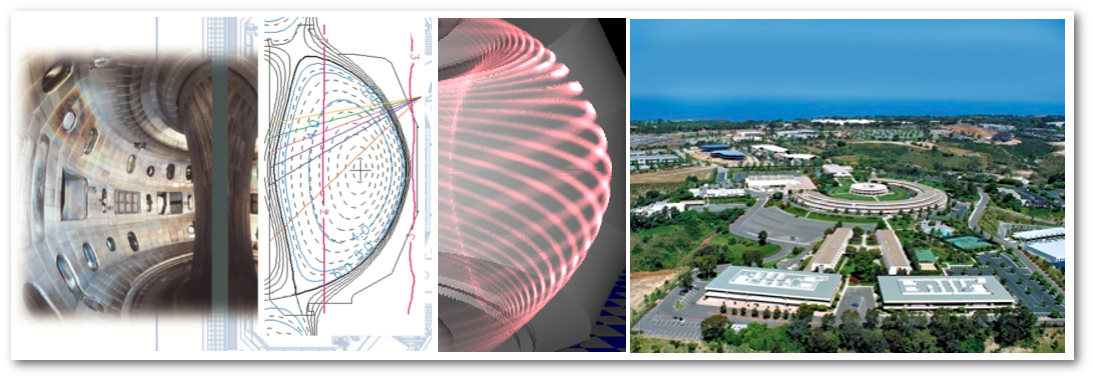
\includegraphics[width=6.8in]{add.png}

General Atomics invites applications for a postdoctoral scholar in magnetic
confinement plasma physics with focus on one of more of the following areas:
(a) plasma kinetic theory and transport including energetic particle dynamics,
(b) fluid and kinetic descriptions of plasma edge physics,
(c) tokamak integrated and predictive modeling.
The candidate should demonstrate general theoretical competence with plasma
equilibrium, stability and kinetic theory.  The candidate should be self-motivated
and creative, but also able to function effectively in a team environment.
Experience with Unix/Linux, Python and Fortran would be advantageous.

If interested, please send CV to Phil Snyder (snyder@fusion.gat.com),
Lang Lao (lao@fusion.gat.com) and Jeff Candy (candy@fusion.gat.com).

\end{document}

